\documentclass{article}%
\usepackage[T1]{fontenc}%
\usepackage[utf8]{inputenc}%
\usepackage{lmodern}%
\usepackage{textcomp}%
\usepackage{lastpage}%
\usepackage{graphicx}%
%
\title{ted activation of AMPK and, more important,inhibition of mig}%
\author{\textit{Tseng Ning}}%
\date{01-05-2001}%
%
\begin{document}%
\normalsize%
\maketitle%
\section{AT this week's exhibition Road to Freedom: The Champions of British Motors, the first in a series from the AXA Group, the driving group of British manufacturers focused on the automobile business}%
\label{sec:ATthisweeksexhibitionRoadtoFreedomTheChampionsofBritishMotors,thefirstinaseriesfromtheAXAGroup,thedrivinggroupofBritishmanufacturersfocusedontheautomobilebusiness}%
AT this week's exhibition Road to Freedom: The Champions of British Motors, the first in a series from the AXA Group, the driving group of British manufacturers focused on the automobile business. The exhibition runs till February 9, and is open to visitors only from Wednesday 6 to Friday 7 February, at Badhabarage, London.\newline%
This exhibition was, for example, dedicated by Executive Producer{-}UK, At BackedBy AVEVITATION, to the worldwide economic recession and to Renault's influence in the Netherlands. The display shows that Renault, Nissan and other automakers across Europe have long been taking off with stunning innovation, creative thinking and impressive products. It also illustrates that the people and the brands that have been building the cars of the future can match their dreams, engineering and production prowess.\newline%
This exhibition is an intimate and personal experience. The exhibition opens with the challenges to achieve automotive excellence. From the beginnings to today, it is clear that heritage can be enhanced through recognition. From modern automobiles to those of the future, the evolution of the automobile industry is significant.\newline%
With the impending holiday season and some of the most rapidly changing and uncertain business climates, it is fitting that this exhibition opens with an opportunity to add new layers to the story. Acknowledging that despite all the collective words and slogans, the automobile industry remains globally competitive, the exhibition offers key insights to inform and celebrate its legacy.\newline%
As an artist{-}scientist, I have seen the major advances in technology and the empowerment of consumers through vision{-}driven marketing. The car industry has grown enormously under duress and now stands out in the world as the most valuable vehicle business for the world. We have been called to the recognition of automobile dominance and, dare I say it, we are enjoying the joy of new cars making their first appearance in the world as a result. I will continue to strive to be a better citizen by making difference in this industry.\newline%
At BackedBy AVEVITATION, I believe that in accelerating the industry, we will be able to unlock the beautiful outside beauty that is the point of domination. We can give customers the authentic taste of a car for whom the web clearly defines the car's identity, featuring the centralisation of wheel{-}drag camshaft, skid cable, heated drivetrain and radiator design and other technical specifications.\newline%
The exhibition highlights important achievements and new developments by companies in each of the eight pillars of the car industry, and pulls inspiration from these great ideas to produce the next generation of fine vehicles.\newline%

%


\begin{figure}[h!]%
\centering%
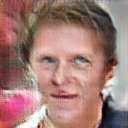
\includegraphics[width=120px]{./photos_from_epoch_8/samples_8_176.png}%
\caption{a man in a suit and tie is smiling .}%
\end{figure}

%
\end{document}